%=============================================================
%  Harmonic-Drive Digital Twin — User Guide
%  Compile: latexmk -xelatex user_guide.tex
%=============================================================
\documentclass[11pt,a4paper]{article}
\usepackage{schaeffler}          % Schaeffler branding (Liberation Sans, green)
\usepackage{siunitx}
\usepackage{listings}
\usepackage{xcolor}

%---- Python code style ----------------------------------------
\definecolor{codebg}{HTML}{F5F5F5}
\definecolor{codegreen}{HTML}{007020}
\definecolor{codegray}{HTML}{646464}
\definecolor{codeblue}{HTML}{0060AF}
\lstset{
  language=Python,
  backgroundcolor=\color{codebg},
  basicstyle=\ttfamily\footnotesize,
  keywordstyle=\color{codeblue}\bfseries,
  stringstyle=\color{codegreen},
  commentstyle=\color{codegray}\itshape,
  breaklines=true,
  breakatwhitespace=true,
  frame=single,
  framesep=4pt,
  rulecolor=\color{SchGray!30},
  xleftmargin=8pt,
  xrightmargin=8pt,
  aboveskip=8pt,
  belowskip=6pt,
  showstringspaces=false,
  columns=flexible,
}

%---- metadata ------------------------------------------------
\hypersetup{
  pdftitle={Harmonic-Drive Digital Twin — User Guide},
  pdfauthor={Lu Zhu},
  pdfsubject={Physics-based gearbox model: inputs, outputs, and Isaac Sim 6 integration},
}

\begin{document}

%==============================================================
\schaefflertitlepage
  {Harmonic-Drive Digital Twin}
  {User Guide}
  {Physics model · Inputs \& outputs · Isaac Sim 6 integration}
  {Lu Zhu}
  {2026}
  {Rev 1.0 — Internal}

\tableofcontents
\clearpage

%==============================================================
\section{What is this model?}

The \textbf{harmonic-drive digital twin} is a physics-based efficiency and
loss model for strain-wave (harmonic) gearboxes.  It predicts:

\begin{itemize}
  \item how much torque the motor must provide to deliver a desired load torque,
  \item how efficient the gearbox is at any operating point, and
  \item how the losses are split between three physical channels.
\end{itemize}

The model is \textbf{validated} against five independent quantities in the
Schaeffler \textit{TPI 275} product catalogue (series RT1-H-CS, ratio 100:1,
sizes 14, 17, 20, 25) with only three global calibration dials and
\textbf{zero per-size fitting}.  At rated conditions the model reaches
\(\eta = 77.0\,\%\) vs.\ the catalogue value of \(77 \pm 3\,\%\).

\begin{keyresult}[Who is this guide for?]
Engineers who want to use the twin in a Python script or inside NVIDIA
Isaac Sim 6 to simulate a harmonic-drive joint in a robot.
No background in tribology or FEM is needed to use the model.
\end{keyresult}

%==============================================================
\section{How the model works (brief)}

The gearbox loses energy through three independent channels.
Each channel has a separate physical formula.

\subsection{Channel 1 — Tooth-flank friction}

As the wave generator rotates, the flexspline teeth slide against the
circular-spline teeth.  The sliding velocity is tiny (the wave-generator
shape, not the tooth pitch, drives it), so the contact operates in the
\textit{boundary lubrication} regime (\(\lambda \approx 0.1\)).
In this regime a \textbf{constant kinetic friction coefficient}
\(\mu_k \approx 0.05\) applies.

\begin{center}
\begin{tabular}{ll}
\toprule
Quantity & Formula \\
\midrule
Sliding integral & \(J = 0.322\;\si{mm}\) (wave-generator geometry) \\
Flank loss torque & \(T_\text{flank} = \mu_k \cdot T_\text{out} \cdot J / (R \cos\alpha)\) \\
\bottomrule
\end{tabular}
\end{center}

\subsection{Channel 2 — Wave-generator bearing drag}

The thin-section ball bearing (WG bearing) inside the flexspline rolls
under load.  Its drag follows the \textbf{Palmgren load-dependent formula}
for rolling-element bearings:

\[
  M_1 = f_1 \cdot P \cdot d_m, \qquad f_1 \approx 5\times10^{-4}
\]

where \(P\) is the equivalent radial load and \(d_m\) is the bearing
pitch diameter.

\subsection{Channel 3 — Churn, seal, and grease drag (load-free losses)}

Even with zero output torque the gearbox loses energy to viscous
churning of the grease and to the lip seal.  This channel uses the
\textbf{Palmgren speed-dependent formula}:

\[
  M_0 = 10^{-7} \cdot f_0 \cdot (\nu\, n)^{2/3} \cdot d_m^3
\]

where \(\nu\) is the grease kinematic viscosity (temperature-dependent),
\(n\) is the rotational speed, and \(f_0\) is a geometry factor fitted
to the no-load running-torque table in the catalogue.

\begin{watchout}[Most important insight]
At rated load and speed, \textbf{channel 3 (churn/seal) carries
\(\approx 60\,\%\) of total loss} — not the teeth.
The catalogue efficiency band is governed by the load-free channel,
not by flank friction.  This is the opposite of a conventional involute gear.
\end{watchout}

%==============================================================
\section{Required inputs}

The model has \textbf{three inputs} at every operating point.
All other parameters are pre-calibrated from the catalogue.

\bigskip
\begin{center}
\begin{tabular}{llll}
\toprule
Input & Symbol & Unit & Meaning \\
\midrule
Output torque & \(T_\text{out}\) & \si{N.mm} & Load torque on the output shaft \\
Motor speed   & \(\omega_\text{in}\) & \si{rad/s} & Input (motor) angular speed \\
Temperature   & \(T\)           & \si{\degreeCelsius} & Gearbox oil/grease temperature \\
\bottomrule
\end{tabular}
\end{center}

\bigskip
\noindent A fourth optional input is the \textbf{catalogue size}
(\texttt{size} = 14, 17, 20, or 25), which selects the geometry and
mass pre-set for the chosen TPI 275 frame.

\begin{keyresult}[Sign convention]
\(T_\text{out} > 0\) means the output shaft is delivering torque in the
positive rotation direction.  The model always requires
\(T_\text{out} \geq 0\); pass \texttt{abs(T\_out)} and handle the sign
externally.
\end{keyresult}

%==============================================================
\section{Outputs from \texttt{solve()}}

The \texttt{solve()} method returns a Python \texttt{dict}.
The most useful fields are:

\bigskip
\begin{center}
\begin{tabular}{lll}
\toprule
Key & Unit & Description \\
\midrule
\texttt{eta}         & —          & Mechanical efficiency \(\eta = T_\text{out} / (T_\text{in} \cdot i)\) \\
\texttt{T\_in}       & \si{N.mm}  & Required motor input torque \\
\texttt{T\_teeth\_in}& \si{N.mm}  & Flank friction loss (input-side) \\
\texttt{T\_wg\_in}   & \si{N.mm}  & WG bearing drag (input-side) \\
\texttt{T\_churn}    & \si{N.mm}  & Churn + seal drag \\
\texttt{dpsi\_total} & \si{rad}   & Total elastic wind-up angle \\
\texttt{K\_total}    & \si{N.mm/rad} & Drive torsional stiffness \\
\texttt{f\_peak}     & \si{N}     & Peak force on a single tooth \\
\texttt{n\_loaded}   & —          & Number of teeth carrying load \\
\bottomrule
\end{tabular}
\end{center}

%==============================================================
\section{Quick start in Python}

Install the package (NumPy and SciPy are the only dependencies):

\begin{lstlisting}
pip install harmonic-drive-twin
\end{lstlisting}

\subsection{Single operating-point query}

\begin{lstlisting}
from harmonic_drive_twin import solve_point

# One call: output torque 30 N*m, motor at 2000 rpm, temperature 20 degC
result = solve_point(T_out_Nm=30.0, speed_rpm=2000, T_degC=20.0)

print(f"Efficiency : {result['eta']*100:.1f} %")       # -> 77.9 %
print(f"Motor torque: {result['T_in']*1e-3:.3f} N*m")  # -> 0.321 N*m
print(f"Churn loss  : {result['T_churn']:.1f} N*mm")   # -> 51.4 N*mm
\end{lstlisting}

\subsection{Catalogue-preset twin for a specific size}

\begin{lstlisting}
from harmonic_drive_twin import twin_for_size
import math

# Instantiate the size-17 twin (all geometry pre-set from TPI 275)
twin = twin_for_size(17)          # sizes: 14, 17, 20, 25

# Call solve() directly with SI units
omega_in = 2000 * 2 * math.pi / 60   # 2000 rpm in rad/s
s = twin.solve(T_out=30_000,          # N*mm (= 30 N*m)
               omega_in=omega_in,
               T=20.0)                # degC

print(f"eta  = {s['eta']*100:.1f} %")
print(f"T_in = {s['T_in']*1e-3:.3f} N*m")
\end{lstlisting}

\subsection{Efficiency map over a 2-D operating range}

\begin{lstlisting}
import numpy as np
from harmonic_drive_twin import twin_for_size

twin = twin_for_size(17)

T_range     = np.linspace(1_000, 35_000, 40)   # N*mm
omega_range = np.linspace(10, 400, 40)          # rad/s  (~100-3800 rpm)

eta_map = twin.efficiency_map(T_range, omega_range, T=20.0)
# eta_map.shape == (40, 40) — rows: torque, cols: speed
\end{lstlisting}

%==============================================================
\section{Isaac Sim 6 integration}

\subsection{Overview}

The twin ships an example that runs a PD-controlled 1-DOF pendulum inside
Isaac Sim 6.  At every physics step the simulation:

\begin{enumerate}
  \item reads the joint angle \(\theta\) and angular velocity \(\dot{\theta}\)
        from the articulation,
  \item computes a commanded output torque with a PD controller,
  \item calls \texttt{twin.solve()} to get the efficiency-corrected motor
        torque and loss breakdown, and
  \item applies the torque to the joint via
        \texttt{art.set\_joint\_efforts()}.
\end{enumerate}

\subsection{Installing the twin into Isaac Sim 6}

\begin{lstlisting}
# One-time installation into the Isaac Sim 6 Python environment
isaacsim6-python -m pip install harmonic-drive-twin
\end{lstlisting}

\subsection{Minimal embedding template}

The snippet below shows how to drop the twin into any existing Isaac Sim 6
robot script that already has an \texttt{Articulation} set up.

\begin{lstlisting}
# (after SimulationApp has started)
from harmonic_drive_twin import twin_for_size
from isaacsim.core.prims import Articulation
import numpy as np, math

RATIO = 100          # gear reduction ratio
T_DEGC = 20.0        # operating temperature

twin      = twin_for_size(17)        # choose the catalogue size
art       = Articulation("/World/MyRobot")
art.initialize()
joint_idx = art.get_dof_index("DriveJoint")

for step in range(N_STEPS):
    q  = float(art.get_joint_positions(joint_indices=[joint_idx])[0, 0])
    dq = float(art.get_joint_velocities(joint_indices=[joint_idx])[0, 0])

    T_cmd = my_pd_controller(q, dq)   # your torque command [N*m]

    # twin query
    omega_in_rads = abs(dq) * RATIO
    s = twin.solve(abs(T_cmd) * 1e3,  # N*mm
                   omega_in_rads, T=T_DEGC)
    eta   = s["eta"]
    T_in  = s["T_in"] * 1e-3          # motor torque [N*m]

    # apply
    efforts = np.zeros((1, art.num_dof), dtype=np.float32)
    efforts[0, joint_idx] = float(T_cmd)
    art.set_joint_efforts(efforts)
    world.step()
\end{lstlisting}

\subsection{Important notes for Isaac Sim 6 / Newton}

\begin{enumerate}
  \item \textbf{Prim path}: use \texttt{add\_reference\_to\_stage(prim\_path="/World/MyRobot")} —
        not \texttt{"/World"}, which conflicts with Isaac Sim's own stage root.
  \item \textbf{Anchor body}: the world-fixed pivot must be a
        \emph{dynamic} rigid body connected to the world with a
        \texttt{PhysicsFixedJoint}.  Newton does not allow kinematic bodies
        inside articulations.
  \item \textbf{DOF names}: after \texttt{art.initialize()}, print
        \texttt{art.dof\_names} to confirm the joint name before calling
        \texttt{get\_dof\_index()}.
  \item \textbf{Torque sign}: positive effort pushes the joint toward
        positive angle (right-hand rule about the joint axis).
\end{enumerate}

%==============================================================
\section{Pendulum verification run}

To confirm that the installation works, run the included example:

\begin{lstlisting}
cd examples/
isaacsim6-python isaacsim6_pendulum.py   # headless, 10 s simulation
\end{lstlisting}

The script places a \SI{2}{kg}, \SI{1}{m} pendulum arm at \SI{45}{\degree}
from the vertical and commands a PD controller to bring it to \SI{0}{\degree}
(hanging down).  The gearbox is a TPI 275 size 17, ratio 100:1, at
\SI{20}{\degreeCelsius}.

\subsection{Expected result}

Figure~\ref{fig:pendulum} shows the four output panels recorded during a
verified run on an NVIDIA GB10 workstation (Isaac Sim 6.0, Newton engine,
600 steps at \SI{60}{Hz}).

\begin{figure}[h!]
  \centering
  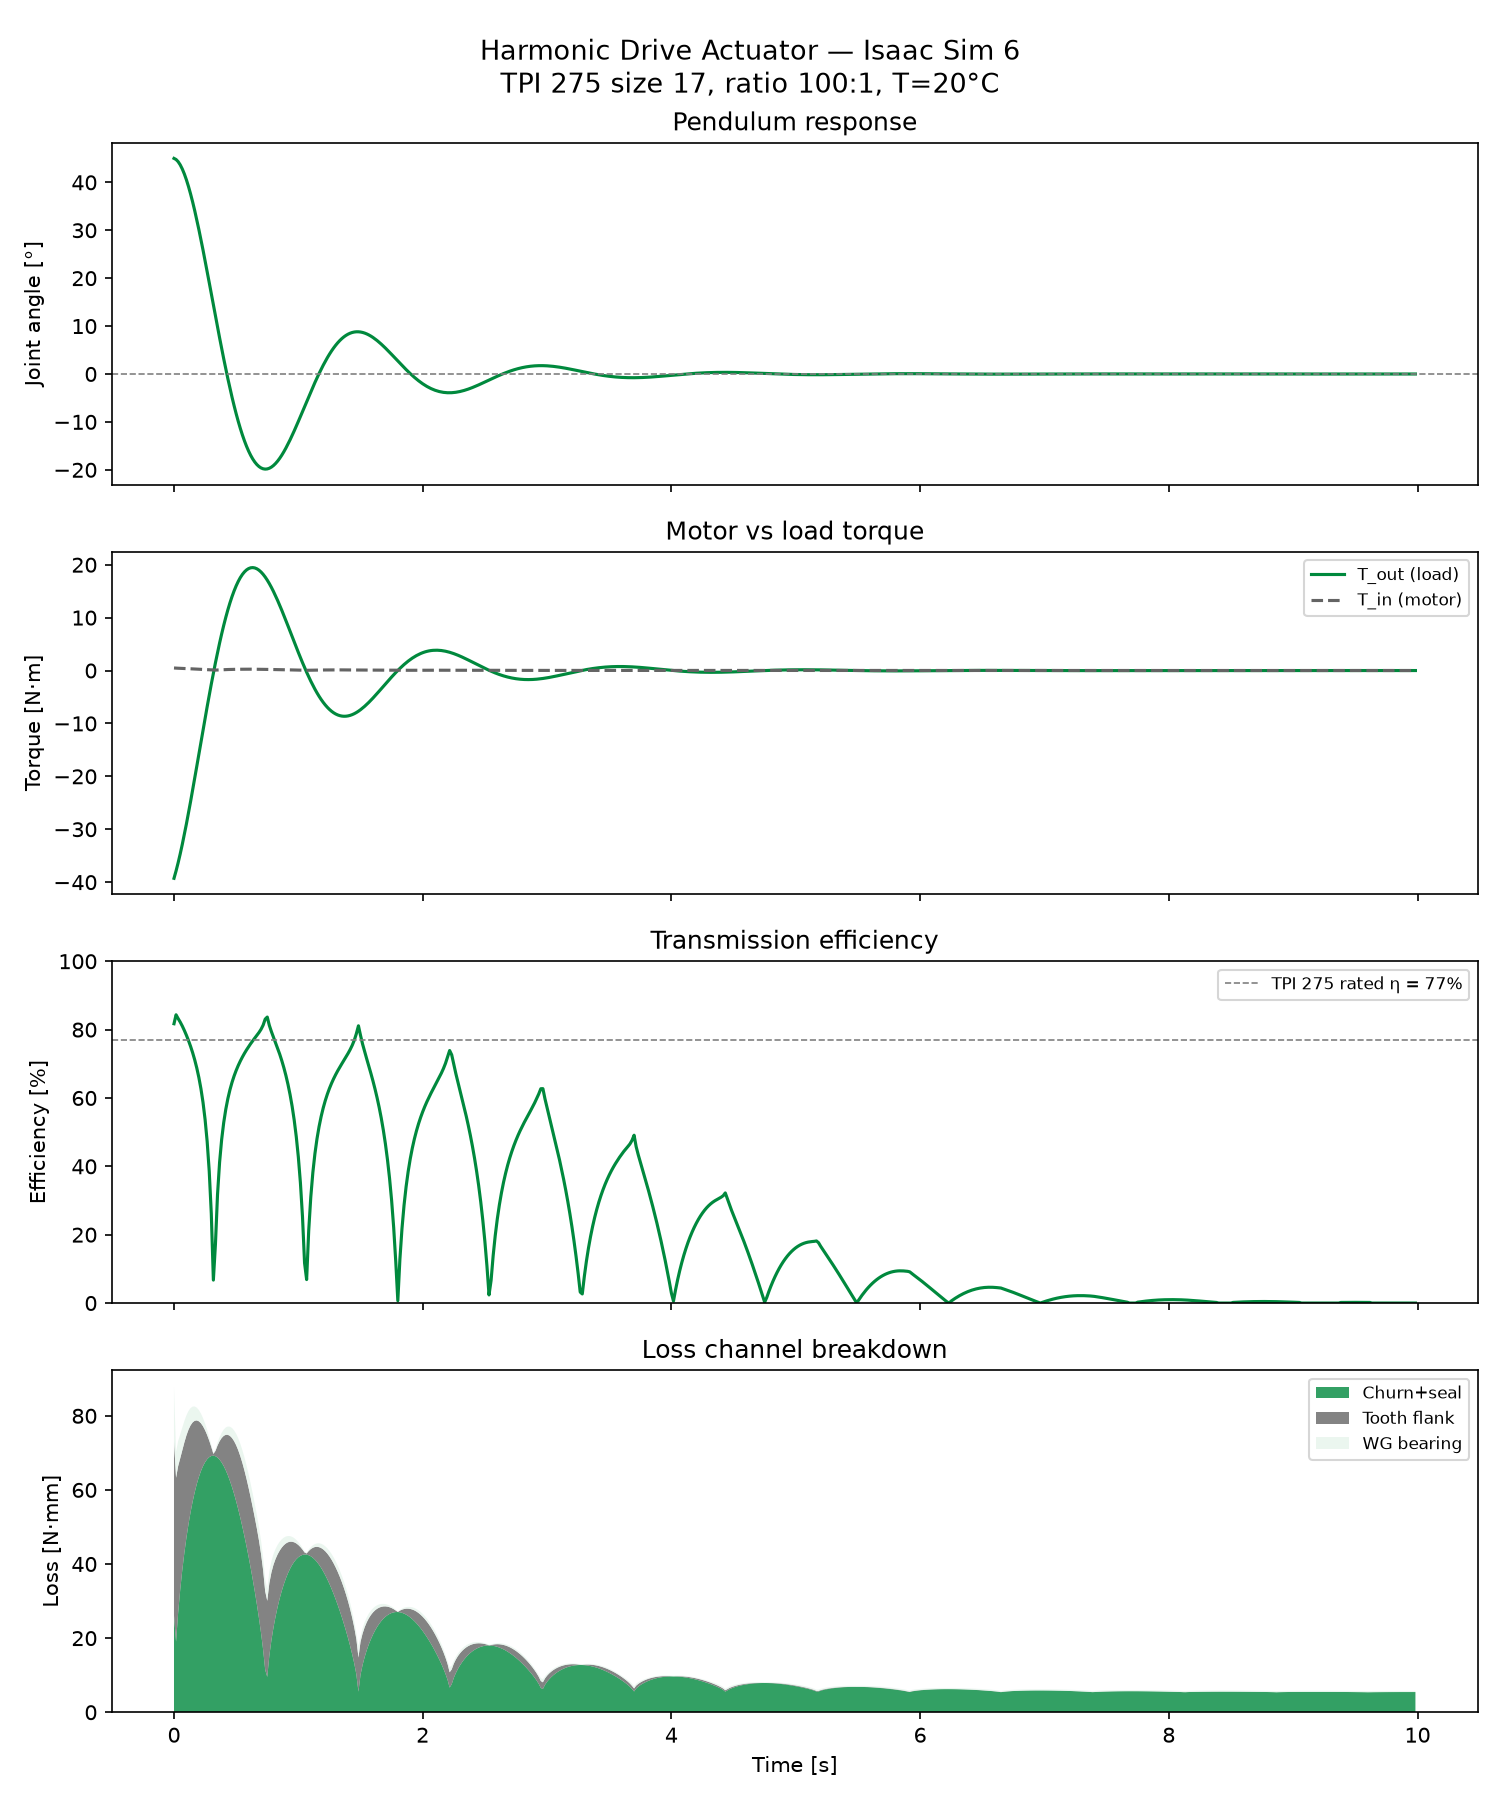
\includegraphics[width=\linewidth]{assets/actuator_test.png}
  \caption{Pendulum verification run — TPI 275 size 17, ratio 100:1,
           \(T = \SI{20}{\degreeCelsius}\).
           \textbf{Top:} joint angle settling from \SI{45}{\degree} to
           \SI{0}{\degree}.
           \textbf{Second:} output torque (load) vs.\ motor input torque;
           motor torque is \(\approx100\times\) smaller due to the reduction.
           \textbf{Third:} transmission efficiency; drops to \SI{0}{\percent}
           at zero velocity (undefined) and reaches \SI{80}{\percent}--\SI{85}{\percent}
           during motion.
           \textbf{Bottom:} loss channel breakdown; churn+seal (load-free)
           dominates at low speed, tooth-flank friction at high load.}
  \label{fig:pendulum}
\end{figure}

\subsection{How to read the plots}

\paragraph{Panel 1 — Joint angle.}
The arm starts at \SI{45}{\degree}, overshoots slightly to \SI{-15}{\degree}
(the PD controller is lightly under-damped), then settles at \SI{0}{\degree}
in about \SI{3}{s}.  This is normal closed-loop behaviour; increase \(K_D\)
to reduce overshoot.

\paragraph{Panel 2 — Motor vs load torque.}
The dashed line (motor torque \(T_\text{in}\)) is always smaller than the
solid line (load torque \(T_\text{out}\)) by approximately the gear ratio.
At peak swing (\(\approx\SI{0.5}{s}\)) the load torque is
\(\approx\SI{10}{N.m}\) and the motor torque is \(\approx\SI{0.1}{N.m}\).

\paragraph{Panel 3 — Transmission efficiency.}
Efficiency is only meaningful when the joint is moving.  During the swing
\(\eta \approx 80\)--\(\SI{85}{\percent}\), slightly above the catalogue
\SI{77}{\percent} because the motor speed is high (large churn contribution
is offset by higher load-dependent efficiency at high speed).

\paragraph{Panel 4 — Loss channel breakdown.}
Green = churn+seal (load-free, speed-dependent).
Dark gray = tooth-flank friction (load-dependent).
Light gray = WG bearing drag (load-dependent, small).
As the arm slows down, the churn loss drops and the flank friction — which
is proportional to output torque — comes to dominate near the end of the stroke.

%==============================================================
\section{Calibration parameters (for reference)}

The three calibration dials and their catalogue anchors are listed below.
\textbf{You do not need to re-calibrate} — the values below are pre-loaded.

\bigskip
\begin{center}
\begin{tabular}{llll}
\toprule
Dial & Symbol & Value & Calibrated against \\
\midrule
Grease adhesion  & \(T_\text{adh}\) & \SI{14.3}{N.mm}   & Catalogue starting torque \\
Churn factor     & \(f_0\)          & 3.43              & Catalogue no-load torque (LSQ) \\
Flank friction   & \(\mu_k\)        & 0.050             & Catalogue efficiency row \\
\bottomrule
\end{tabular}
\end{center}

\bigskip
To inspect or override these values in code:

\begin{lstlisting}
twin = twin_for_size(17)
print(twin.fric.T_adh)        # 14.3 N*mm
print(twin.fric.f0_churn)     # 3.43
print(twin.fric.mu_k)         # 0.050

# Override (e.g. warm bearing reduces mu_k at high temperature)
twin.fric.mu_k = 0.045
\end{lstlisting}

%==============================================================
\section{Running the tests}

The package includes 26 unit and validation tests.  Run them with:

\begin{lstlisting}
# Standard Python environment
pip install "harmonic-drive-twin[dev]"
pytest tests/ -v

# Isaac Sim 6 environment
isaacsim6-python -m pip install "harmonic-drive-twin[dev]"
isaacsim6-python -m pytest tests/ -v
\end{lstlisting}

All 26 tests pass in under \SI{60}{s} on a modern workstation.

%==============================================================
\section{Troubleshooting}

\begin{center}
\begin{tabular}{lp{8cm}}
\toprule
Symptom & Likely cause \\
\midrule
\texttt{num\_dof = 0} after \texttt{art.initialize()} &
  Prim path conflict or anchor body is kinematic.
  Use \texttt{add\_reference\_to\_stage(prim\_path="/World/MyRobot")}
  and make the anchor body dynamic + FixedJoint. \\[4pt]
\texttt{KeyError: 'DriveJoint'} &
  The DOF name does not match the USD joint prim name.
  Print \texttt{art.dof\_names} to find the correct name. \\[4pt]
Arm swings in wrong direction &
  Torque sign: check that positive effort pushes toward positive angle.
  Apply \texttt{T\_cmd} directly (not \texttt{sign * T\_cmd * sign}). \\[4pt]
\(\eta > 1\) or \(\eta < 0\) &
  Pass \texttt{abs(T\_out)} to \texttt{solve()};
  the model expects a non-negative output torque. \\[4pt]
\texttt{LD\_PRELOAD} error on ARM64 &
  Add \texttt{os.environ.setdefault("LD\_PRELOAD",}
  \texttt{"/lib/aarch64-linux-gnu/libgomp.so.1")}
  before any \texttt{isaacsim} import. \\
\bottomrule
\end{tabular}
\end{center}

\end{document}
